
\chapter{Running PyLith}

Figure \vref{fig:pylith:workflow} shows the workflow for running PyLith.
There are essentially three main inputs needed to run a problem with
PyLith:
\begin{enumerate}
\item Mesh information. This includes the topology of the
  finite-element mesh (coordinates of vertices and how the vertices
  are connected into cells), a material identifier for each cell, and
  sets of vertices associated with boundary conditions, faults, and
  output (for subsets of the mesh). This information can be provided
  using the PyLith mesh ASCII format (see Chapter \vref{cha:examples}
  for examples and Section \vref{sec:format:MeshIOAscii} for the format
  specification) or by importing the information from the LaGriT or
  CUBIT meshing packages (see Chapter \vref{cha:examples} for
  examples).
\item A set of parameters describing the problem. These parameters
  describe the type of problem to be run, solver information,
  time-stepping information, boundary conditions, materials, etc. This
  information can be provided from the command-line or by using a
  \filename{.cfg.}
\item Databases specifying the material property values and boundary
  condition values to be used. Arbitrarily complex spatial variations
  in boundary and fault conditions and material properties may be
  given in the spatial database (see Chapter \vref{cha:examples} for
  examples and Appendix \vref{sec:format:SimpleIOAscii} for the
  format specification).
\end{enumerate}
PyLith writes solution information, such as solution fields and state
variables, to either VTK files or HDF5/Xdmf files. ParaView and Visit
can read both types of files. Post-processing of output is generally
performed using HDF5 files accessed via a Python script and the h5py
package or a Matlab script.

\begin{figure}[htbp]
  \includegraphics[width=5in]{runpylith/figs/runpylith} 
  \caption{PyLith requires a finite-element mesh (three different
    mechanisms for generating a mesh are currently supported),
    simulation parameters, and spatial databases (defining the spatial
    variation of various parameters).  PyLith writes the solution
    output to either VTK or HDF5/Xdmf files, which can be visualized
    with ParaView or Visit. Post-processing is generally done using
    the HDF5 files with Python or Matlab scripts.}
\label{fig:pylith:workflow} 
\end{figure}

% ----------------------------------------------------------------------
\section{Defining the Simulation}

The parameters for PyLith are specified as a hierarchy or tree of
modules. The application assembles the hierarchy of modules from user
input and then calls the \object{main} function in the top-level
module in the same manner as a C or C++ program. The behavior of the
application is determined by the modules included in the hierarchy as
specified by the user. The Pyre framework provides the interface for
defining this hierarchy. Appendix \vref{cha:components} contains a
list of the components provided by PyLith and spatialdata.

Pyre properties correspond to simple settings in the form of strings,
integers, and real numbers. Pyre facilities correspond to software
modules. Facilities may have their own facilities (branches in the
tree) and any number of properties. See Figure
\vref{fig:Pyre:architecture} for the general concept of Pyre
facilities and properties.

\subsection{Setting PyLith Parameters}
\label{sec:setting:parameters}

There are several methods for setting input parameters for the
\filename{pylith} executable: via the command line or by using a text
file in \filename{cfg} or \filename{pml} format. Both facilities and
properties have default values provided, so you only need to set
values when you want to deviate from the default behavior.


\subsubsection{Units}

All dimensional parameters require units. The units are specified
using Python syntax, so square meters is m**2. Whitespace is not
allowed in the string, for units and dimensioned quantities are
multiplied by the units string; for example, two meters per second is
2.0*m/s. Available units are shown in Table \vref{tab:pyre:units}

\begin{table}[htbp]
\caption{Pyre supported units. Aliases are in parentheses.}
\label{tab:pyre:units}
\begin{tabular}{lp{5in}}
\textbf{Scale} & \textbf{Available Units} \\
\hline 
length & meter (m), micrometer (um, micron), millimeter (mm), centimeter (cm),
kilometer (km), inch, foot, yard, mile \\
time & second (s), nanosecond (ns), microsecond (us), millisecond (ms), minute,
hour, day, year \\
mass & kilogram (kg), gram (g), centigram (cg), milligram (mg), ounce, pound,
ton \\
pressure & pascal (Pa), kPa, MPa, GPa, bar, millibar, atmosphere (atm) \\
\hline 
\end{tabular}
\end{table}


\subsubsection{Using the Command Line}

The \commandline{-{}-help} command line argument displays links to useful
resources for learning PyLith.

Pyre uses the following syntax to change properties from the command
line. To change the value of a property of a component, use
\commandline{-{}-COMPONENT.PROPERTY=VALUE}. Each component is attached
to a facility, so the option above can also be written as
\commandline{-{}-FACILITY.PROPERTY=VALUE}.  Each facility has a
default component attached to it. A different component can be
attached to a facility by \commandline{-{}-FACILITY=NEW\_COMPONENT}.

PyLith's command-line arguments can control Pyre and PyLith properties
and facilities, MPI settings, and PETSc settings. All PyLith-related
properties are associated with the \facility{pylithapp} component. You
can get a list of all of these top-level properties along with a
description of what they do by running PyLith with the
\commandline{-{}-help-properties} command-line argument. To get
information on user-configurable facilities and components, you can
run PyLith with the \commandline{-{}-help-components} command-line
argument. To find out about the properties associated with a given
component, you can run PyLith with the
\commandline{-{}-COMPONENT.help-properties} flag:
\begin{shell}
$ pylith --problem.help-properties

# Show problem components.
$ pylith --problem.help-components

# Show bc components (bc is a component of problem).
$ pylith --problem.bc.help-components

# Show bc properties.
$ pylith --problem.bc.help-properties
\end{shell}


\subsubsection{Using a {\ttfamily .cfg} File}

Entering all those parameters via the command line involves the risk
of typographical errors. You
will generally find it easier to collect parameters into a
\filename{cfg} file. The file is composed of one or more sections
which are formatted as follows:
\begin{cfg}
<h>[pylithapp.COMPONENT1.COMPONENT2]</h>
# This is a comment.

<f>FACILITY3</f> = COMPONENT3
<p>PROPERTY1</p> = VALUE1
<p>PROPERTY2</p> = VALUE2 ; this is another comment
\end{cfg}

\tip{We strongly recommend that you use \filename{cfg} files for your
  work.  The files are syntax-highlighted in most editors, such as
  vim, Emacs, and Atom.}


\subsubsection{Using a {\ttfamily.pml} File}

A \filename{pml} file is an XML file that specifies parameter values
in a highly structured format. It is composed of nested sections which
are formatted as follows:
\begin{lstlisting}[basicstyle=\ttfamily,frame=tb]{language=xml}
<component~name="COMPONENT1">
    <component~name="COMPONENT2">
        <property~name="PROPERTY1">VALUE1</property>
        <property~name="PROPERTY2">VALUE2</property>
    </component>
</component>
\end{lstlisting}
XML files are intended to be read and written by machines, not edited
manually by humans. The \filename{pml} file format is intended for
applications in which PyLith input files are generated by another
program, e.g., a GUI, web application, or a high-level structured
editor. This file format will not be discussed further here, but if
you are interested in using \filename{pml} files, note that \filename{pml}
files and \filename{cfg} files can be used interchangeably; in the
following discussion, a file with a \filename{pml} extension can be
substituted anywhere a \filename{cfg} file can be used.


\subsubsection{Specification and Placement of Configuration Files}

Configuration files may be specified on the command line:
\begin{shell}
$ pylith example.cfg
\end{shell}
In addition, the Pyre framework searches for configuration files named
\filename{pylithapp.cfg} in several predefined locations. You may put
settings in any or all of these locations, depending on the scope
you want the settings to have:
\begin{enumerate}
\item \filename{\$PREFIX/etc/pylithapp.cfg}, for system-wide settings;
\item \filename{\$HOME/.pyre/pylithapp/pylithapp.cfg}, for user
  settings and preferences;
\item the current directory (\filename{./pylithapp.cfg}), for local
  overrides.
\end{enumerate}

\important{The Pyre framework will search these directories for
  \filename{cfg} files matching the names of components (for example,
  \filename{timedependent.cfg}, \filename{faultcohesivekin.cfg},
  \filename{greensfns.cfg}, \filename{pointforce.cfg}, etc) and will
  attempt to assign all parameters in those files to the respective
  component.}

\important{Parameters given directly on the command line will override
  any input contained in a configuration file. Configuration files
  given on the command line override all others. The
  \filename{pylithapp.cfg} files placed in (3) will override those in
  (2), (2) overrides (1), and (1) overrides only the built-in
  defaults.}

All of the example problems are set up using configuration files and specific problems are defined by including
the appropriate configuration file on the command-line. Referring
to the directory \filename{examples/twocells/twohex8}, we have the
following.
\begin{shell}
$ ls -1 *.cfg
axialdisp.cfg
dislocation.cfg
pylithapp.cfg
sheardisp.cfg
\end{shell}
The settings in \filename{pylithapp.cfg} will be read automatically, and additional
settings are included by specifying one of the other files on the
command-line:
\begin{shell}
$ pylith axialdisp.cfg
\end{shell}
If you want to see what settings are being used, you can either examine
the \filename{cfg} files, or use the help flags as described above:
\begin{shell}
# Show components for the 'problem' facility.
$ pylith axialdisp.cfg --problem.help-components

# Show properties for the 'problem' facility.
$ pylith axialdisp.cfg --problem.help-properties

# Show components for the 'bc' facility.
$ pylith axialdisp.cfg --problem.bc.help-components

# Show properties for the 'bc' facility.
$ pylith axialdisp.cfg --problem.bc.help-properties
\end{shell}
This is generally a more useful way of determining problem settings,
since it includes default values as well as those that have been specified
in the \filename{cfg} file.


\subsubsection{List of PyLith Parameters (\filename{pylith\_info})}
\label{sec:pylithinfo}

The Python application \filename{pylith\_info} writes all of the current
parameters to a text file or JSON file (default). The default name of the JSON is \filename{pylith\_parameters.json}.
The usage synopsis is
\begin{shell}
$ pylith_info [--verbose-false] [--format={ascii,json} [--filename=pylith_parameters.json] PYLITH_ARGS
\end{shell}
where \commandline{-{}-verbose-false} turns off printing the descriptions of
the properties and components as well as the location where the
current value was set, \commandline{-{}-format=ascii} changes the
output format to a simple ASCII file, and \\
\commandline{-{}-filename=pylith\_parameters.json} sets the name of the
output file. The PyLith Parameter Viewer (see Section
\ref{sec:pylith:parameter:viewer}) provides a graphic user interface
for examining the JSON parameter file. 


% End of file

\section{Time-Dependent Problem (\facilityshape{formulation})}

This type of problem applies to transient static, quasi-static, and
dynamic simulations. The time-dependent problem adds the
\facility{formulation} facility to the general-problem. The
formulation specifies the time-stepping formulation to integrate the
elasticity equation. PyLith provides several alternative formulations,
each specific to a different type of problem.
\begin{description}
\item[\object{Implicit}] Implicit time stepping for static and
   quasi-static problems with infinitesimal strains. The implicit
   formulation neglects inertial terms (see Section
   \vref{eq:elasticity:integral:quasistatic}).
\item[\object{ImplicitLgDeform}] Implicit time stepping for static
  and quasi-static problems including the effects of rigid body motion
  and small strains.  This formulation requires the use of the
  nonlinear solver, which is selected automatically.
\item[\object{Explicit}] Explicit time stepping for dynamic problems
  with infinitesimal strains and lumped system Jacobian. The cell
  matrices are lumped before assembly, permitting use of a vector for
  the diagonal system Jacobian matrix. The built-in lumped solver is
  selected automatically.
\item[\object{ExplicitLgDeform}] Explicit time stepping for dynamic
  problems including the effects of rigid body motion and small
  strains. The cell matrices are lumped before assembly, permitting
  use of a vector for the diagonal system Jacobian matrix. The
  built-in lumped solver is selected automatically.
\item[\object{ExplicitTri3}] Optimized elasticity formulation for
  linear triangular cells with one point quadrature for dynamic
  problems with infinitesimal strains and lumped system Jacobian. The
  built-in lumped solver is selected automatically.
\item[\object{ExplicitTet4}] Optimized elasticity formulation for
  linear tetrahedral cells with one point quadrature for dynamic
  problems with infinitesimal strains and lumped system Jacobian. The
  built-in lumped solver is selected automatically.
\end{description}
In many quasi-static simulations it is convenient to compute a static
problem with elastic deformation prior to computing a transient response.
Up through PyLith version 1.6 this was hardwired into the Implicit
Forumulation as advancing from time step $t=-\Delta t$ to $t=0$,
and it could not be turned off. PyLith now includes a property, \property{elastic\_prestep}
in the TimeDependent component to turn on/off this behavior (the default
is to retain the previous behavior of computing the elastic deformation).

\warning{Turning off the elastic
prestep calculation means the model only deforms when an {\it increment}
in loading or deformation is applied, because the time-stepping formulation
is implemented using the increment in displacement.}

The \object{TimeDependent} properties and facilities include
\begin{inventory}
  \propertyitem{elastic\_preset}{If true, perform a static calculation with elastic
    behavior before time stepping (default is True).}
  \facilityitem{formulation}{Formulation for solving the partial differential
    equation.}
\end{inventory}
An example of setting the properties and components in a \filename{.cfg} file
is
\begin{cfg}
<h>[pylithapp.timedependent]</h>
<f>formulation</f> = pylith.problems.Implicit ; default
<f>progres_monitor</f> = pylith.problems.ProgressMonitorTime ; default
<p>elastic_preset</p> = True ; default
\end{cfg}
The formulation value can be set to the other formulations in a similar
fashion. 


\subsection{Time-Stepping Formulation}

The explicit and implicit time stepping formulations use a common
set of facilities and properties. The properties and facilities include
\begin{inventory}
\propertyitem{matrix\_type}{Type of PETSc matrix for the system Jacobian (sparse
matrix, default is symmetric, block matrix with a block size of 1).}
\propertyitem{view\_jacobian}{Flag to indicate if system Jacobian (sparse matrix)
should be written to a file (default is false).}
\propertyitem{split\_fields}{Split solution field into a displacement portion
(fields 0..ndim-1) and a Lagrange multiplier portion (field ndim)
to permit application of sophisticated PETSc preconditioners (default
is false).}
\facilityitem{time\_step}{Time step size specification (default is \object{TimeStepUniform} (uniform time step).}
\facilityitem{solver}{Type of solver to use (default is \object{SolverLinear}).}
\facilityitem{output}{Array of output managers for output of the solution (default
is [output]).}
\facilityitem{jacobian\_viewer}{Viewer to dump the system Jacobian (sparse matrix)
to a file for analysis (default is PETSc binary).}
\end{inventory}

An example of setting these parameters in a \filename{.cfg} file is
\begin{cfg}
<h>[pylithapp.timedependent.formulation]</h>
<p>matrix_type</p> = sbaij ; Non-symmetric sparse matrix is 'aij'
<p>view_jacobian</p> = false

# Nonlinear solver is pylith.problems.SolverNonlinear
<f>solver</f> = pylith.problems.SolverLinear
<f>output</f> = [domain, ground_surface]
<f>time_step</f> = pylith.problems.TimeStepUniform
\end{cfg}

\subsection{Numerical Damping in Explicit Time Stepping}

In explicit time-stepping formulations for elasticity, boundary conditions
and fault slip can excite short waveform elastic waves that are not
accurately resolved by the discretization. We use numerical damping
via an artificial viscosity\cite{Knopoff:Ni:2001,Day:Ely:2002} to
reduce these high frequency oscillations. In computing the strains
for the elasticity term in equation \vref{eq:elasticity:integral:dynamic:t},
we use an adjusted displacement rather than the actual displacement,
where 
\begin{equation}
\vec{u}^{adj}(t)=\vec{u}(t)+\eta^{*}\Delta t\vec{\dot{u}}(t),
\end{equation}
$\vec{u}^{adj}(t)$ is the adjusted displacement at time t, $\vec{u}(t)$is
the original displacement at time (t), $\eta^{*}$is the normalized
artificial viscosity, $\Delta t$ is the time step, and $\vec{\dot{u}}(t)$
is the velocity at time $t$. The default value for the normalized
artificial viscosity is 0.1. We have found values in the range 0.1-0.4
sufficiently suppress numerical noise while not excessively reducing
the peak velocity. An example of setting the normalized artificial
viscosity in a \filename{.cfg} file is
\begin{cfg}
<h>[pylithapp.timedependent.formulation]</h>
<p>norm_viscosity</p> = 0.2
\end{cfg}

\subsection{Solvers}
\label{sec:solvers}

PyLith supports three types of solvers. The linear solver,
SolverLinear, corresponds to the PETSc KSP solver and is used in
linear problems with linear elastic and viscoelastic bulk constitutive
models and kinematic fault ruptures. The nonlinear solver,
SolverNonlinear, corresponds to the PETSc SNES solver and is used in
nonlinear problems with nonlinear viscoelastic or elastoplastic bulk
constitutive models, dynamic fault ruptures, or problems involving
finite strain (small strain formulation).  The lumped solver
(SolverLumped) is a specialized solver used with the lumped system
Jacobian matrix. The options for the PETSc KSP and SNES solvers are
set via the top-level PETSc options (see Section
\vref{sec:petsc:options} and the PETSc documentation
\url{www.mcs.anl.gov/petsc/petsc-as/documentation/index.html}).


\subsection{Time Stepping}
\label{sub:Time-Stepping}

PyLith provides three choices for controlling the time step in time-dependent
simulations. These include (1) a uniform, user-specified time step
(which is the default), (2) user-specified time steps (potentially
nonuniform), and (3) automatically calculated (potentially nonuniform)
time steps. The procedure for automatically selecting time steps requires
that the material models provide a reasonable estimate of the time
step for stable time integration. In general, quasi-static simulations
with viscoelastic materials should use automatically calculated time
steps and dynamic simulations should use a uniform, user-specified
time step. Note that all three of the time stepping schemes make use
of the computed stable time step (see \vref{sec:stable:time:step}).
When using user-specified time steps, the value is checked against
the computed stable time step. The automatically calculated time step
comes from the computed stable time step.

\warning{Varying the time step within a simulation requires
  recomputing the Jacobian of the system whenever the time step
  changes, which can greatly increase the runtime if the time-step
  size changes frequently.}

\subsubsection{Uniform, User-Specified Time Step (\object{TimeStepUniform})}

With a uniform, user-specified time step, the user selects the time
step that is used over the entire duration of the simulation. If this
value exceeds the computed stable time step at any time, PyLith will
terminate with an error. The properties for the uniform, user-specified
time step are:
\begin{inventory}
\propertyitem{total\_time}{Time duration for simulation (default is 0.0 s).}
\propertyitem{start\_time}{Start time for simulation (default is 0.0 s).}
\propertyitem{dt}{Time step for simulation.}
\end{inventory}
An example of setting a uniform, user-specified time step in a \filename{.cfg}
file is:
\begin{cfg}
<h>[pylithapp.problem.formulation]</h>
<p>time_step</p> = pylith.problems.TimeStepUniform ; Default value

<h>[pylithapp.problem.formulation.time_step]</h>
<p>total_time</p> = 1000.0*year
<p>dt</p> = 0.5*year
\end{cfg}

\subsubsection{Nonuniform, User-Specified Time Step (\object{TimeStepUser})}

The nonuniform, user-specified, time-step implementation allows the
user to specify the time steps in an ASCII file (see Section
\vref{sec:format:timestepuser} for the format specification of the
time-step file). If the total duration exceeds the time associated
with the time steps, then a flag determines whether to cycle through
the time steps or to use the last specified time step for the time
remaining. Similar to the uniform time step, if the user-specified
time step size exceeds the computed stable time step at any time,
PyLith will terminate with an error.  The properties for the
nonuniform, user-specified time step are:
\begin{inventory}
\propertyitem{total\_time}{Time duration for simulation.}
\propertyitem{filename}{Name of file with time-step sizes.}
\propertyitem{loop\_steps}{If true, cycle through time steps, otherwise keep
using last time-step size for any time remaining.}
\end{inventory}
An example of setting the properties for nonuniform, user-specified
time steps in a \filename{.cfg} file is:
\begin{cfg}
<h>[pylithapp.problem.formulation]</h>
<f>time_step</f> = pylith.problems.TimeStepUser ; Change the time step algorithm

<h>[pylithapp.problem.formulation.time_step]</h>
<p>total_time</p> = 1000.0*year
<p>filename</p> = timesteps.txt
<p>loop_steps</p> = false ; Default value
\end{cfg}

\subsubsection{Nonuniform, Automatic Time Step (\object{TimeStepAdapt})}

This time-step implementation automatically calculates a time step
size based on the constitutive model and rate of deformation. As a
result, this choice for choosing the time step relies on accurate
calculation of a stable time step within each finite-element cell
by the constitutive models. To provide some control over the time-step
selection, the user can control the frequency with which a new time
step is calculated, the time step to use relative to the value determined
by the constitutive models, and a maximum value for the time step.
Note that the stability factor allows the computed time step size
to exceed the computed stable time step. A stability factor of 1.0
would provide a time step size equal to the stable time step, while
a value of 2.0 (default value) would provide a time step size equal
to 1/2 the stable time step. Caution should be used when adjusting
the stability factor to values less than 1.0, as the large time step
size may result in inaccurate solutions. The properties for controlling
the automatic time-step selection are:
\begin{inventory}
\propertyitem{total\_time}{Time duration for simulation.}
\propertyitem{max\_dt}{Maximum time step permitted.}
\propertyitem{adapt\_skip}{Number of time steps to skip between calculating
new stable time step.}
\propertyitem{stability\_factor}{Safety factor for stable time step (default
is 2.0).}
\end{inventory}
An example of setting the properties for the automatic time step in
a \filename{.cfg} file is:
\begin{cfg}
<h>[pylithapp.problem.formulation]</h>
<p>time_step</p> = pylith.problems.TimeStepAdapt ; Change the time step algorithm

<h>[pylithapp.problem.formulation.time_step]</h>
<p>total_time</p> = 1000.0*year
<p>max_dt</p> = 10.0*year
<p>adapt_skip</p> = 10 ; Default value
<p>stability_factor</p> = 2.0 ; Default value
\end{cfg}

\section{Green's Functions Problem (\object{GreensFns})}

This type of problem applies to computing static Green's functions
for elastic deformation. The \object{GreensFns} problem specializes
the time-dependent facility to the case of static simulations with
slip impulses on a fault. The default formulation is the Implicit
formulation and should not be changed as the other formulations are
not applicable to static Green's functions. In the output files, the
deformation at each ``time step'' is the deformation for a different
slip impulse. The properties provide the ability to select which fault
to use for slip impulses. The only fault component available for use
with the \object{GreensFns} problem is the \object{FaultCohesiveImpulses}
component discussed in Section \vref{sec:fault:cohesive:impulses}.
The \object{GreensFns} properties amd facilities include:
\begin{inventory}
\propertyitem{fault\_id}{Id of fault on which to impose slip impulses.}
\propertyitem{formulation}{Formulation for solving the partial differential
equation.}
\propertyitem{progress\_monitor}{Simple progress monitor via text file.}
\end{inventory}
An example of setting the properties for the GreensFns problem in
a \filename{.cfg} file is:
\begin{cfg}
<h>[pylithapp]</h>
<f>problem</f> = pylith.problems.GreensFns ; Change problem type from the default

<h>[pylithapp.greensfns]</h>
<p>fault_id</p> = 100 ; Default value
<f>formulation</f> = pylith.problems.Implicit ; default
<f>progres_monitor</f> = pylith.problems.ProgressMonitorTime ; default
\end{cfg}

\warning{The \object{GreensFns} problem generates slip impulses on a
  fault. The current version of PyLith requires that impulses can only
  be applied to a single fault and the fault facility must be set to
  \object{FaultCohesiveImpulses}.}

\section{Progress Monitors}
\newfeature{v2.1.0}

The progress monitors make it easy to monitor the general progress of
long simulations, especially on clusters where stdout is not always
easily accessible. The progress monitors update a simulation's current
progress by writing information to a text file. The information
includes time stamps, percent completed, and an estimate of when the
simulation will finish.

\subsection{\object{ProgressMonitorTime}}

This is the default progress monitor for time-stepping problems. The
monitor calculates the percent completed based on the time at the
current time step and the total simulated time of the simulation,
not the total number of time steps (which may be unknown in simulations
with adaptive time stepping). The \object{ProgressMonitorTime} properties
include:
\begin{inventory}
\propertyitem{update\_percent}{Frequency (in percent) of progress updates.}
\propertyitem{filename}{Name of output file.}
\propertyitem{t\_units}{Units for simulation time in output.}
\end{inventory}
An example of setting the properties in a \filename{.cfg} file is:
\begin{cfg}
<h>[pylithapp.problem.progressmonitor]</h>
<p>update_percent</p> = 5.0 ; default
<p>filename</p> = progress.txt ; default
<p>t_units</p> = year ; default
\end{cfg}

\subsection{\object{ProgressMonitorStep}}

This is the default progress monitor for problems with a specified
number of steps, such as Green's function problems. The monitor calculates
the percent completed based on the number of steps (e.g., Green's
function impulses completed). The ProgressMonitorStep propertiles
include:
\begin{inventory}
\propertyitem{update\_percent}{Frequency (in percent) of progress updates.}
\propertyitem{filename}{Name of output file.}
\end{inventory}
An example of setting the properties in a \filename{.cfg} file is:
\begin{cfg}
<h>[pylithapp.problem.progressmonitor]</h>
<p>update_percent</p> = 5.0 ; default
<p>filename</p> = progress.txt ; default
\end{cfg}

% End of file
\section{Databases for Boundaries, Interfaces, and Material Properties}
\label{sec:spatial:databases}

Once the problem has been defined with PyLith parameters, and the
mesh information has been provided, the final step is to specify the
boundary conditions and material properties to be used. The mesh information
provides labels defining sets of vertices to which boundary conditions
or fault conditions will be applied, as well as cell labels that will
be used to define the material type of each cell. For boundary conditions,
the \filename{.cfg} file is used to associate boundary condition types
and spatial databases with each vertex group (see Chapter \vref{cha:boundary:interface:conditions}).
For materials, the \filename{.cfg} file is used to associate material
types and spatial databases with cells identified by the material
identifier (see Figure \vref{fig:material:models}).

The spatial databases define how the boundary conditions or material
property values vary spatially, and they can be arbitrarily complex.
The simplest example for a material database would be a mesh where
all the cells of a given type have uniform properties (``point''
or 0D variation). A slightly more complex case would be a mesh where
the cells of a given type have properties that vary linearly along
a given direction (``line'' or 1D variation). In more complex models,
the material properties might have different values at each point
in the mesh (``volume'' or 3D variation). This might be the case,
for example, if the material properties are provided by a database
of seismic velocities and densities. For boundary conditions the simplest
case would be where all vertices in a given group have the same boundary
condition parameters (``point'' or 0D variation). A more complex
case might specify a variation in the conditions on a given surface
(``area'' or 2D variation). This sort of condition might be used,
for example, to specify the variation of slip on a fault plane. The
examples discussed in Chapter \vref{cha:examples} also contain more
information regarding the specification and use of the spatial database
files.


\subsection{\object{SimpleDB} Spatial Database}

In most cases the default type of spatial database for faults, boundary
conditions, and materials is \object{SimpleDB}. Spatial database files
provide specification of a field over some set of points. There is
no topology associated with the points. Although multiple values can
be specified at each point with more than one value included in a
search query, the interpolation of each value will be done independently.
Time dependent variations of a field are not supported in these files.
Spatial database files can specify spatial variations over zero, one,
two, and three dimensions. Zero dimensional variations correspond
to uniform values. One-dimensional spatial variations correspond to
piecewise linear variations, which need not coincide with coordinate
axes. Likewise, two-dimensional spatial variations correspond to variations
on a planar surface (which need not coincide with the coordinate axes)
and three-dimensional spatial variations correspond to variations
over a volume. In one, two, or three dimensions, queries can use a
``nearest value'' search or linear interpolation.

The spatial database files need not provide the data using the same
coordinate system as the mesh coordinate system, provided the two
coordinate systems are compatible. Examples of compatible coordinate
systems include geographic coordinates (longitude/latitude/elevation),
and projected coordinates (e.g., coordinates in a transverse Mercator
projection). Spatial database queries use the Proj.4 Cartographic
Projections library \url{proj.maptools.org} to convert between coordinate
systems, so a large number of geographic projections are available
with support for converting between NAD27 and WGS84 horizontal datums
as well as several other frequently used datums. Because the interpolation
is done in the coordinate system of the spatial database, geographic
coordinates should only be used for very simple datasets, or undesirable
results will occur. This is especially true when the spatial database
coordinate system combines latitude, longitude, and elevation in meters
(longitude and latitude in degrees are often much smaller than elevations
in meters leading to distorted ``distance'' between locations and
interpolation).

\object{SimpleDB} uses a simple ASCII file to specify the variation of values (e.g., displacement field, slip field, physical properties) in space.  The file format is described in Section \vref{sec:spatialdata:SimpleIOAscii}.  The tutorials in Chapter \vref{cha:examples} use \object{SimpleDB} files to specify the values for the boundary conditions, physical properties, and fault slip.

As in the other Pyre objects, spatial database objects contain parameters
that can be set from the command line or using \filename{.cfg}
files. The properties and facilities for a spatial database are:
\begin{inventory}
\propertyitem{label}{Label for the database, which is used in diagnostic messages.}
\propertyitem{query\_type}{Type of search query to perform. Values for this
parameter are ``linear'' and ``nearest'' (default).}
\facilityitem{iohandler}{Database importer. Only one importer is implemented,
so you do not need to change this setting.}
\propertyitem{iohandler.filename}{Filename for the spatial database.}
\end{inventory}
An example of setting these in a \filename{.cfg} file is:
\begin{cfg}
<p>label</p> = Material properties
<p>query_type</p> = linear
<p>iohandler.filename</p> = mydb.spatialdb
\end{cfg}

\subsection{\object{UniformDB} Spatial Database}

The \object{SimpleDB} spatial database is quite general, but when the values
are uniform, it is often easier to use the \object{UniformDB} spatial database
instead. With the \object{UniformDB}, you specify the values directly either
on the command line or in a parameter-setting (\filename{.cfg}) file.
On the other hand, if the values are used in more than one place,
it is easier to place the values in a \object{SimpleDB} file, because they
can then be referred to using the filename of the spatial database
rather than having to repeatedly list all of the values on the command
line or in a parameter-setting (\filename{.cfg}) file. The properties
for a \object{UniformDB} are:
\begin{inventory}
\propertyitem{values}{Array of names of values in spatial database.}
\propertyitem{data}{Array of values in spatial database.}
\end{inventory}

Specify the physical properties of a linearly elastic, isotropic material
in a \filename{.cfg} file. The data values are dimensioned
with the appropriate units using Python syntax.
\begin{cfg}
<h>[pylithapp.timedependent.materials.material]</h>
<p>db_properties</p> = spatialdata.spatialdb.UniformDB ; Set the db to a UniformDB
<p>db_properties.values</p> = [vp, vs, density] ; Set the names of the values in the database
<p>db_properties.data</p> = [5773.5*m/s, 3333.3*m/s, 2700.0*kg/m**3] ; Set the values in the database}
\end{cfg}

\subsubsection{\object{ZeroDispDB}}

The \object{ZeroDispDB} is a special case of the \object{UniformDB} for the Dirichlet
boundary conditions. The values in the database are the ones requested
by the Dirichlet boundary conditions, \filename{displacement-x}, \filename{displacement-y},
and \filename{displacement-z}, and are all set to zero. This makes it
trivial to set displacements to zero on a boundary. The examples discussed
in Chapter \vref{cha:examples} use this database.


\subsection{\object{SimpleGridDB} Spatial Database}

The \object{SimpleGridDB} object provides a much more efficient query
algorithm than \object{SimpleDB} in cases with a orthogonal grid. The
points do not need to be uniformly spaced along each coordinate
direction. Thus, in contrast to the \object{SimpleDB} there is an
implicit topology. Nevertheless, the points can be specified in any
order, as well as over a lower-dimension than the spatial dimension.
For example, one can specify a 2-D grid in 3-D space provided that the
2-D grid is aligned with one of the coordinate axes.

\object{SimpleGridDB} uses a simple ASCII file to specify the variation of
values (e.g., displacement field, slip field, physical properties) in
space. The file format is described in Section
\vref{sec:spatialdata:SimpleGrid}.

As in the other Pyre objects, spatial database objects contain parameters
that can be set from the command line or using \filename{.cfg}
files. The parameters for a spatial database are:
\begin{inventory}
\propertyitem{label}{Label for the database, which is used in
  diagnostic messages.}
\propertyitem{query\_type}{Type of search query to perform. Values for this
parameter are ``linear'' and ``nearest'' (default).}
\propertyitem{filename}{Filename for the spatial database.}
\end{inventory}
An example of setting these parameters in a \filename{.cfg} file is:
\begin{cfg}
<p>label</p> = Material properties
<p>query_type</p> = linear
<p>filename</p> = mydb_grid.spatialdb
\end{cfg}

\subsection{SCEC CVM-H Spatial Database (\object{SCECCVMH})}
\label{sec:SCEC:CVM-H}

Although the \object{SimpleDB} implementation is able to specify arbitrarily
complex spatial variations, there are existing databases for physical
properties, and when they are available, it is desirable to access
these directly. One such database is the SCEC CVM-H database, which
provides seismic velocities and density information for much of southern
California. Spatialdata provides a direct interface to this database.
See Section \vref{sec:examples:twotet4-geoproj} for an example of
using the SCEC CVM-H database for physical properties of an elastic
material. The interface is known to work with versions 5.2 and 5.3
of the SCEC CVM-H. Setting a minimum wave speed can be used to replace
water and very soft soils that are incompressible or nearly incompressible
with stiffer, compressible materials. The Pyre properties for the
SCEC CVM-H are:
\begin{inventory}
\propertyitem{data\_dir}{Directory containing the SCEC CVM-H data
  files.}
\propertyitem{min\_vs}{Minimum shear wave speed. Corresponding minimum values
for the dilatational wave speed (Vp) and density are computed. Default
value is 500 m/s.}
\propertyitem{squash}{Squash topography/bathymetry to sea level (make the earth's
surface flat).}
\propertyitem{squash\_limit}{Elevation above which topography is squashed (geometry
below this elevation remains undistorted).}
\end{inventory}

Specify the physical properties of a linearly elastic, isotropic material
using the SCEC CVM-H in a \filename{.cfg} file.
\begin{cfg}
<h>[pylithapp.timedependent.materials.material]</h>
<p>db_properties</p> = spatialdata.spatialdb.SCECCVMH ; Set the database to the SCEC CVM-H

# Directory containing the database data files.
<p>db_properties.data_dir</p> = /home/johndoe/data/sceccvm-h/vx53

<p>db_properties.min_vs</p> = 500*m/s ; Default value
<p>db_properties.squash</p> = True ; Turn on squashing

# Only distort the geometry above z=-1km in flattening the earth
<p>db_properties.squash_limit</p> = -1000.0
\end{cfg}

\subsection{\object{CompositeDB} Spatial Database}

For some problems, a boundary condition or material property may have
subsets with different spatial variations. One example would be when
we have separate databases to describe the elastic and inelastic bulk
material properties for a region. In this case, it would be useful
to have two different spatial databases, e.g., a seismic velocity
model with Vp, Vs, and density values, and another database with the
inelastic physical properties. We can use the \object{CompositeDB}
spatial database for these cases. An example would be:
\begin{cfg}
<h>[pylithapp.timedependent.materials.maxwell]</h>
<p>label</p> = Maxwell material
<p>id</p> = 1
<f>db_properties</f> = spatialdata.spatialdb.CompositeDB
<f>db_properties.db_A</f> = spatialdata.spatialdb.SCECCVMH
<f>db_properties.db_B</f> = spatialdata.spatialdb.SimpleDB
<f>quadrature.cell</f> = pylith.feassemble.FIATSimplex
<p>quadrature.cell.dimension</p> = 3

<h>[pylithapp.timedependent.materials.maxwell.db_properties]</h>
<p>values_A</p> = [density, vs, vp]
<p>db_A.label</p> = Elastic properties from CVM-H
<p>db_A.data_dir</p> = /home/john/tools/vx53/bin
<p>db_A.squash</p> = False
<p>values_B</p> = [viscosity]
<p>db_B.label</p> = Vertically varying Maxwell material
<p>db_B.iohandler.filename<p> = ../spatialdb/mat_maxwell.spatialdb
\end{cfg}
Here we have specified a \object{CompositeDB} where the elastic properties
(density, vs, vp) are given by the SCEC
CVM-H, and viscosity is described by a \object{SimpleDB}
(\filename{mat\_maxwell.spatialdb}). The user must first
specify \facility{db\_properties} as a \object{CompositeDB}, and must
then give the two components of this database (in this case, \object{SCECCVMH} and
\object{SimpleDB}). The values to query in each of these databases
is also required. This is followed by the usual parameters for each
of the spatial databases. The \object{CompositeDB} provides a flexible
mechanism for specifying material properties or boundary conditions
where the variations come from two different sources.


\subsection{\object{TimeHistory} Database}

The \object{TimeHistory} database specifies the temporal variation in the
amplitude of a field associated with a boundary condition. It is used
in conjunction with spatial databases to provide spatial and temporal
variation of parameters for boundary conditions. The same time history
is applied to all of the locations, but the time history may be shifted
with a spatial variation in the onset time and scaled with a spatial
variation in the amplitude. The time history database uses a simple
ASCII file which is simpler than the one used by the \object{SimpleDB} spatial
database. The file format is described in Section \vref{sec:Spatialdata:TimeHistoryIO}. 

As in the other Pyre objects, spatial database objects contain parameters
that can be set from the command line or using \filename{.cfg}
files. The parameters for a spatial database are:
\begin{inventory}
\propertyitem{label}{Label for the time history database, which is used in diagnostic
messages.}
\propertyitem{filename}{Filename for the time history database.}
\end{inventory}
An example of setting these parameters in a \filename{.cfg} file is:
\begin{cfg}
<p>label</p> = Displacement time history
<p>filename</p> = mytimehistory.timedb
\end{cfg}

% End of file
\section{Labels and Identifiers for Materials, Boundary Conditions, and Faults}

For materials, the ``label'' is a string used only for error messages.
The ``id'' is an integer that corresponds to the material identifier
in LaGriT (itetclr) and CUBIT/Trelis (block id). The id also tags the
cells in the mesh for associating cells with a specific material model
and quadrature rule. For boundary conditions, the ``label'' is a
string used to associate groups of vertices (psets in LaGriT and
nodesets in CUBIT/Trelis) with a boundary condition. Some mesh
generators use strings (LaGriT) to identify groups of nodes while
others (CUBIT/Trelis) use strings and integers. The default behavior
in PyLith is to use strings to identify groups for both LaGriT and
CUBIT/Trelis meshes, but the behavior for CUBIT/Trelis meshes can be
changed to use the nodeset id (see Section \vref{sec:MeshIOCubit}).
PyLith 1.0 had an ``id'' for boundary conditions, but we removed it
from subsequent releases because it was not used. For faults the
``label'' is used in the same manner as the ``label'' for boundary
conditions. That is, it associates a string with a group of vertices
(pset in LaGriT and nodeset in CUBIT/Trelis). The fault ``id'' is a
integer used to tag the cohesive cells in the mesh with a specific
fault and quadrature rule. Because we use the fault ``id'' to tag
cohesive cells in the mesh the same way we tag normal cells to
materials, it must be unique among the faults as well as the
materials.


% End of file

\section{Output}

PyLith currently supports output to HDF5/Xdmf and VTK files, which can
be imported directly into a number of visualization tools, such as
ParaView, Visit, and MayaVi. The HDF5 files can also be directly
accessed via Matlab and Python modules, such as h5py and
PyTables. PyLith v3.x supports output of the solution subfields (see
Section \vref{sec:solution:observers}) all auxiliary fields
(material properties, boundary condition parameters, and fault interface
parameters, etc.) and fields derived from the auxiliary field and/or
solution, such as stress and stress.

HDF5 writer provides parallel binary output, whereas the VTK writer
provides serial ASCII output. Additionally, with the VTK writer each
time step is written to a separate file; the HDF5 writer puts all
information for a given domain, boundary condition, or fault interface
into a single file.


\subsection{Physics Observer (\object{OutputPhysics})}

Analogous to the \object{OutputSoln} objects discussed in Section
\vref{sec:solution:observers} for output of the solution, the physics
objects (material, boundary conditions, and fault interfaces) have
\object{OutputPhysics} objects to provide output of the solution,
properties, state variables, etc. 

The parameters for the \object{OutputPhysics} are:
\begin{inventory}
  \propertyitem{info\_fields}{List of auxiliary subfields to observer/output (default=all which will output all of the subfields);}
  \propertyitem{data\_fields}{List of solution subfields to observer/output (default=all which will output all of the subfields);}
  \facilityitem{writer}{Writer for data (default=\object{DataWriterHDF5});}
  \facilityitem{trigger}{Trigger defining how often output is written (default=\object{OutputTriggerStep}); and}
  \facilityitem{output\_basis\_order}{Basis order for output of
    fields. Valid values are 0 and 1 (default=1).}
\end{inventory}

Fields with a basis order of 0 are kept at a basis order of 0 when output.
Fields with a basis order of 1 are written as vertex fields, whereas fields with a basis order of 0 are written as cell fields.

\begin{cfg}[\object{PhysicsOutput} parameters in a \filename{cfg} file]
<h>[pylithapp.problem.materials.elastic.observers.observer]</h>
<p>writer.filename</p> = output/step01-elastic.h5
<p>output_basis_order</p> = 1
\end{cfg}

\subsection{Data Writers (\facility{writer})}

\subsubsection{VTK Output (\object{DataWriterVTK})}

PyLith writes legacy (non-XML) VTK files. These are simple files with
vertex coordinates, the mesh topology, and fields over vertices and/or
cells. Each time step is written to a different file. The time stamp
is included in the filename with the decimal point removed. This allows
automatic generation of animations with many visualization packages
that use VTK files. The default time stamp is the time in seconds,
but this can be changed using the normalization constant to give a
time stamp in years, tens of years, or any other value.


The parameters for the VTK writer are:
\begin{inventory}
\propertyitem{filename}{Name of VTK file.}
\propertyitem{time\_format}{C-style format string for time stamp in filename.
The decimal point in the time stamp will be removed for compatibility
with VTK visualization packages that provide seamless animation of
data from multiple VTK files.}
\propertyitem{time\_constant}{Value used to normalize time stamp in VTK files
(default is 1.0 s).}
\end{inventory}

\userwarning{We strongly discourage use of using VTK output. It is slow,
  inefficient, and not easily read from post-processing scripts. We
  strongly recommwnd using HDF5 output instead, which is the default
  starting in PyLith v3.0.0.}

\subsubsection{HDF5/Xdmf Output (\object{DataWriterHDF5}, \object{DataWriterHDF5Ext})}
\label{sub:HDF5/Xdmf-Output}

HDF5 files provide a flexible framework for storing simulation data
with datasets in groups logically organized in a tree structure analogous
to files in directories. HDF5 output offers parallel, multi-dimensional
array output in binary files, so it is much faster and more convenient
than the VTK output which uses ASCII files and separate files for
each time step. Standards for organizing datasets and groups in HDF5
files do not exist for general finite-element software in geodynamics.
Consequently, PyLith uses its own simple layout show in Figure \vref{fig:hdf5:layout}.
In order for visualization tools, such as ParaView, to determine which
datasets to read and where to find them in the hierarchy of groups
within the HDF5 file, we create an Xdmf (eXtensible Data Model and
Format, \url{www.xdmf.org}) metadata file that provides this information.
This file is written when PyLith closes the HDF5 file at the end of
the simulation. In order to visualize the datasets in an HDF5 file,
one simply opens the corresponding Xdmf file (the extension is \filename{xmf})
in ParaView or Visit. The Xdmf file contains the relative path to
the HDF5 file so the files can be moved but must be located together
in the same directory. 

\important{The Xdmf format supports
representation of two- and three-dimensional coordinates of points,
scalar fields, and three-dimensional vector and tensor fields but
not two-dimensional vector or tensor fields. Consequently, for two-dimensional
vector fields we build a three-component vector from the two-component
vector (x and y components) and a separate zero scalar field (z component).
For tensor fields, we create a scalar field for each of the tensor
components, adding the component as a suffix to the name of the field.}

\begin{figure}[htbp]
  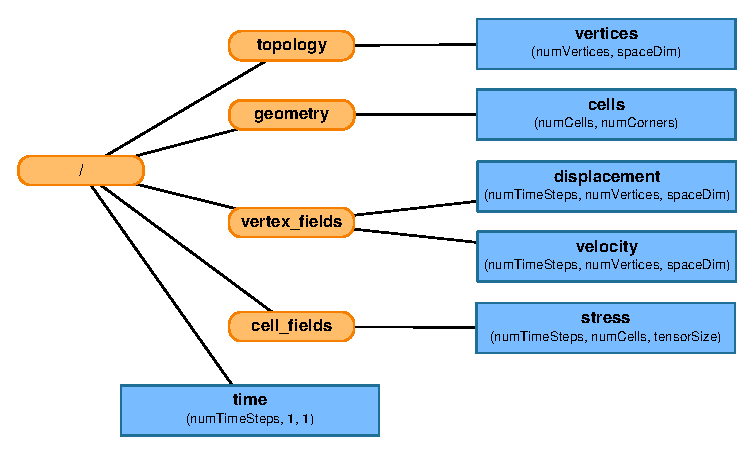
\includegraphics{runpylith/figs/hdf5layout}
  \caption{General layout of a PyLith HDF5 file. The orange rectangles
    with rounded corners identify the groups and the blue rectangles
    with sharp corners identify the datasets. The dimensions of the
    data sets are shown in parentheses. Most HDF5 files will contain
    either \texttt{vertex\_fields} or \texttt{cell\_fields} but not
    both.}
 \label{fig:hdf5:layout}
\end{figure}

See Table \vref{tab:materials:statevars} in Section
\vref{sec:material:parameters} for a table of component values for
tensor output in HDF5 files. To avoid confusion about the ordering of
components for tensor data, we separate the components in the Xdmf
file.

The \object{DataWriterHDF5} and \object{DataWriterHDF5Ext} property is:
\begin{inventory}
  \propertyitem{filename}{Name of HDF5 file (default=output.h5; the
    Xdmf filename is generated from the same prefix).}
\end{inventory}

\begin{cfg}[\object{DataWriterHDF5Ext} parameters in a \filename{cfg} file]
<h>[pylithapp.timedependent.domain.output]</h>
<p>output_freq</p> = time_step
<p>time_step</p> = 1.0*yr
<p>cell_data_fields</p> = [displacement, velocity]
<f>writer</f> = pylith.meshio.DataWriterHDF5Ext
<p>writer.filename</p> = dislocation.h5
\end{cfg}
In this example, we change the writer from the default VTK writer to
the HDF5 writer with external datasets (\object{DataWriterHDF5Ext})
for output over the domain.

HDF5 files do not contain self-correcting features that allow a file
to be read if part of a dataset is corrupted. This type of error can
occur if a job terminates abnormally in the middle or at the end of a
simulation on a large cluster or other parallel machine. Fortunately,
HDF5 also offers the ability to store datasets in external binary
files with the locations specified by links in the HDF5 file. Note
that the use of external data files results in one data file per
dataset in addition to the HDF5 and Xdmf files. The external data
files use the name of the HDF5 file with the dataset name added to the
prefix and the \filename{h5} suffix replaced by \filename{dat}. The
HDF5 files include relative paths to the external data files, so these
files can also be moved, but they, too, must be kept together in the
same directory. This provides a more robust method of output because
one can generate an HDF5 file associated with the uncorrupted portions
of the external data files should an error occur. Currently, PyLith
does not include a utility to do this, but we plan to add one in a
future release. Thus, there are two options when writing PyLith output
to HDF5 files: (1) including the datasets directly in the HDF5 files
themselves using the \object{DataWriterHDF5} object or (2) storing the
datasets in external binary files with just metadata in the HDF5 files
using the \object{DataWriterHDF5Ext} object. Both methods provide
similar performance because they will use MPI I/O if it is available.

\userwarning{Storing the datasets within the HDF5 file in a parallel
  simulation requires that the HDF5 library be configured with the
  \commandline{-{}-enable-parallel} option. The binary PyLith packages
  include this feature and it is a default setting in building HDF5
  via the PyLith Installer.}

Accessing the datasets for additional analysis or visualization is
nearly identical in the two methods because the use of external data
files is completely transparent to the user except for the presence
of the additional files. Note that in order for ParaView to find the
HDF5 and external data files, it must be run from the same relative
location where the simulation was run. For example, if the simulation
was run from a directory called ``work'' and the HDF5/Xdmf files
were written to ``work/output'', then ParaView should be run from
the ``work'' directory. See Table \vref{tab:materials:statevars}
in Section \vref{sec:material:parameters} for a table of component
values for tensor output.

\begin{cfg}[Selecting \object{DataWriterHDF5Ext} in a \filename{cfg}
  file]
<h>[pylithapp.problem]</h>
<f>solution_observers</f> = [domain]
<f>solution_observers.domain>/f> = pylith.mehsio.DataWriterHDF5Ext

<h>[pylithapp.problem.solution_observers.domain]</h>
<p>writer.filename</p> = output/step01-domain.h5
\end{cfg}

\subsubsection{HDF5 Utilities}

HDF5 includes several utilities for examining the contents of HDF5
files. \filename{h5dump} is very handy for dumping the hierarchy,
dimensions of datasets, attributes, and even the dataset values to
stdout. 
\begin{shell}
# Dump the entire HDF5 file (not useful for large files).
$ h5dump mydata.h5

# Dump the hierarchy of an HDF5 file.
$ h5dump -n mydata.h5

# Dump the hierarchy with dataset dimensions and attributes.
$ h5dump -H mydata.h5

# Dump dataset 'vertices' in group '/geometry' to stdout.
$ h5dump -d /geometry/vertices mydata.h5
\end{shell}
We have also include a utility \filename{pylith\_genxdmf} (see Section
\vref{sec:pylith:genxdmf}) that generates an appropriate Xdmf file
from a PyLith HDF5 file. This is very useful if you add fields to
HDF5 files in post-processing and wish to view the results in ParaView
or Visit.


\subsection{Output Triggers (\facility{trigger})}
\newfeature{3.0.0}

By default PyLith will write the requested output after every time
step. In many cases we prefer to save the solution, state variables,
etc at a coarser temporal resolution. The \object{OutputTriggerStep}
controls the decimation of the output by time step, and the
\object{OutputTriggerTime} controls the decimation of the output via
time. For uniform time stepping these are equivalent.

\subsubsection{Decimate by time step (\object{OutputTriggerStep})}

\object{OutputTriggerStep} decimates the output by skipping a
user-specified number of time steps. The property is
\begin{inventory}
  \propertyitem{num\_skip}{Number of solution steps to skip between
    writes (default=0).}
\end{inventory}

  
\subsubsection{Decimate by time (\object{OutputTriggerTime})}

\object{OutputTriggerTime} decimates the output by skipping a
user-specified elasped time. The property is
\begin{inventory}
  \propertyitem{elapsed\_time}{Elasped time between writes (default=0.0*s).}
\end{inventory}
 
\usertip{Due to roundoff error in determining the simulation time over
  many time steps, a simulation may occasionally skip writing output
  unexpectedly when using \object{OutputTriggerTime}. The best
  workaround is to use an \property{elapsed\_time} that is a fraction
  of the time step size smaller than the desired elapsed time, such as
  0.9999*year instead of 1.0*year.}
  
% End of file

\section{Tips and Hints}
\label{sec:tips:hints}

\subsection{Tips and Hints For Running PyLith}
\begin{itemize}
\item Examine the examples for a problem similar to the one you want to
run and dissect it in detail.
\item Start with a uniform-resolution coarse mesh to debug the problem setup.
Increase the resolution as necessary to resolve the solution fields
of interest (resolving stresses/strains may require a higher resolution
than that for resolving displacements).
\item Merge materials using the same material model. This will result in
only one VTK or HDF5 file for each material model rather than several
files.
\item The rate of convergence in quasi-static (implicit) problems can sometimes
be improved by renumbering the vertices in the finite-element mesh
to reduce the bandwidth of the sparse matrix. PyLith can use the reverse
Cuthill-McKee algorithm to reorder the vertices and cells.
\item If you encounter errors or warnings, run \filename{pylithinfo} or use
the \commandline{-{}-help}, \commandline{-{}-help-components}, and \commandline{-{}-help-properties}
command-line arguments when running PyLith to check the parameters
to make sure PyLith is using the parameters you intended.
\item Use the \commandline{-{}-petsc.log\_}view, \commandline{-{}-petsc.ksp\_monitor},
\commandline{-{}-petsc.ksp\_view}, \commandline{-{}-petsc.ksp\_converged\_reason}, and \commandline{-{}-petsc.snes\_converged\_reason}
command-line arguments (or set them in a parameter file) to view PyLith
performance and monitor the convergence.
\item Turn on the journals (see the examples) to monitor the progress of
the code.
\end{itemize}

\subsection{Troubleshooting}
\label{sec:Troubleshooting}

Consult the PyLith FAQ webpage (\url{http://www.geodynamics.org/cig/community/workinggroups/short/workarea/pylith-wiki})
which contains a growing list of common problems and their corresponding
solutions.

\subsubsection{Import Error and Missing Library}
\begin{shell}
ImportError: liblapack.so.2: cannot open shared object file: No such file or directory
\end{shell}

PyLith cannot find one of the libraries. You need to set up your environment
variables (e.g., PATH, PYTHONPATH, and LD\_LIBRARY\_PATH) to match
your installation. If you are using the PyLith binary on Linux or
Mac OS X, run the command \filename{source setup.sh }in the directory
where you unpacked the distribution. This will set up your environment
variables for you. If you are building PyLith from source, please
consult the instructions for building from source.

\subsubsection{Unrecognized Property 'p4wd'}

\begin{shell}
-- pyre.inventory(error) } \\
-- p4wd <- 'true' } \\
-- unrecognized property 'p4wd' } \\
>> command line:: } \\
-- pyre.inventory(error) } \\
-- p4pg <- 'true' } \\
-- unrecognized property ' p4pg'}
\end{shell}
Verify that the filename{mpirun} command included in the PyLith package is
the first one on your PATH: \filename{which mpirun}. If it is not, adjust your PATH environment variable accordingly.

\subsubsection{Detected zero pivor in LU factorization}

\begin{shell}
-- Solving equations.
[0] PETSC ERROR: ----------------
Error Message -------------------------------
[0] PETSC ERROR: Detected zero pivot in LU factorization
see http://www.mcs.anl.gov/petsc/petsc-as/documentation/faq.html\#ZeroPivot!
\end{shell}

This usually occurs when the null space of the system Jacobian is
nonzero, such as the case of a problem without Dirichlet boundary
conditions on any boundary. If this arises when using the split fields
and algebraic multigrid preconditioning, and no additional Dirichlet
boundary conditions are desired, then the workaround is to revert
to using the Additive Schwarz preconditioning without split fields
as discussed in Section \vref{sec:petsc:options}.

\subsubsection{Bus Error}

This often indicates that PyLith is using incompatible versions of
libraries. This can result from changing your environment variables
after configuring or installing PyLith (when building from source) or
from errors in setting the environment variables (\filename{PATH},
\filename{LD\_LIBRARY\_PATH}, and \filename{PYTHONPATH}). If the
former case, simply reconfigure and rebuild PyLith. In the latter
case, check your environment variables (order matters!) to make sure
PyLith finds the desired directories before system directories.

\subsubsection{Segmentation Fault}

A segmentation fault usually results from an invalid read/write to
memory. It might be caused by an error that wasn't trapped or a bug in
the code. Please report these cases so that we can fix these problems
(either trap the error and provide the user with an informative error
message, or fix the bug). If this occurs with any of the problems
distributed with PyLith, simply submit a bug report (see Section
\vref{sec:help}) indicating which problem you ran and your
platform. If the crash occurs for a problem you created, it is a great
help if you can try to reproduce the crash with a very simple problem
(e.g., adjust the boundary conditions or other parameters of one of
the examples to reproduce the segmentation fault). Submit a bug report
along with log files showing the backtrace from a debugger (e.g., gdb)
and the valgrind log file (only available on Linux platforms).  You
can generate a backtrace using the debugger by using the
\commandline{-{}-petsc.start\_in\_debugger} command-line argument:
\begin{shell}
$$ pylith [..args..] --petsc.start_in_debugger
(gdb) continue
(gdb) backtrace
\end{shell}

To use valgrind to detect the memory error, first go to your working
directory and run the problem with \commandline{-{}-launcher.dry}:
\begin{shell}
$$ pylith [..args..] --launcher.dry
\end{shell}

Instead of actually running the problem, this causes PyLith to dump
the mpirun/mpiexec command it will execute. Copy and paste this command
into your shell so you can run it directly. Insert the full path to
valgrind before the full path to mpinemesis and tell valgrind to use
a log file:
\begin{shell}
$$ mpirun /path/to/valgrind --log-file=valgrind-log /path/to/mpinemesis --pyre-start
  [..lots of junk..]
\end{shell}

% End of file

\section{Post-Processing Utilities}

The PyLith distribution includes a few post-processing utilities.
These are Python scripts that are installed into the same bin directory
as the \filename{pylith} executable.


\subsection{\filename{pylith\_eqinfo}}

This utility computes the moment magnitude, seismic moment, seismic
potency, and average slip at user-specified time snapshots from PyLith
fault HDF5 output. The utility works with output from simulations
with either prescribed slip and/or spontaneous rupture. Currently,
we compute the shear modulus from a user-specified spatial database
at the centroid of the fault cells. In the future we plan to account
for lateral variations in shear modulus across the fault when calculating
the seismic moment. The Python script is a Pyre application, so its
parameters can be specified using \filename{.cfg} and command line arguments
just like PyLith. The Pyre properties and facilities include:
\begin{inventory}
\propertyitem{output\_filename}{Filename for output of slip information.}
\propertyitem{faults}{Array of fault names.}
\propertyitem{filename\_pattern}{Filename pattern in C/Python format for creating
filename for each fault. Default is \filename{output/fault\_\%s.h5}.}
\propertyitem{snapshots}{Array of timestamps for slip snapshosts ([-1] means
use last time step in file, which is the default).}
\propertyitem{snapshot\_units}{Units for timestamps in array of snapshots.}
\facilityitem{db\_properties}{Spatial database for elastic properties.}
\facilityitem{coordsys}{Coordinate system associated with mesh in simulation.}
\end{inventory}

\subsection{\filename{pylith\_genxdmf}}
\label{sub:genxdmf}

This utility generates Xdmf files from HDF5 files that conform to
the layout used by PyLith. It is a simple Python script with a single
command line argument, the HDF5 file for input. Typically, it is used
to regenerate Xdmf files that get corrupted or lost due to renaming
and moving. It is also useful in updating Xdmf files when users add
fields to HDF5 files during post-processing.
\begin{shell}
$$ pylith_genxdmf --file=PYLITH_HDF5_FILE
\end{shell}

\warning{If the HDF5 files contain external datasets, then this
  utility should be run from the same relative path to the HDF5 files
  as when they were created. For example, if a PyLith simulation was
  run from directory \filename{work} and HDF5 files were generated in
  \filename{output/work}, then the utility should be run from the
  directory \filename{work}. Furthermore, a visualization tool, such
  as ParaView, should also be started from the working directory
  \filename{work}.}

% End of file

% End of file

